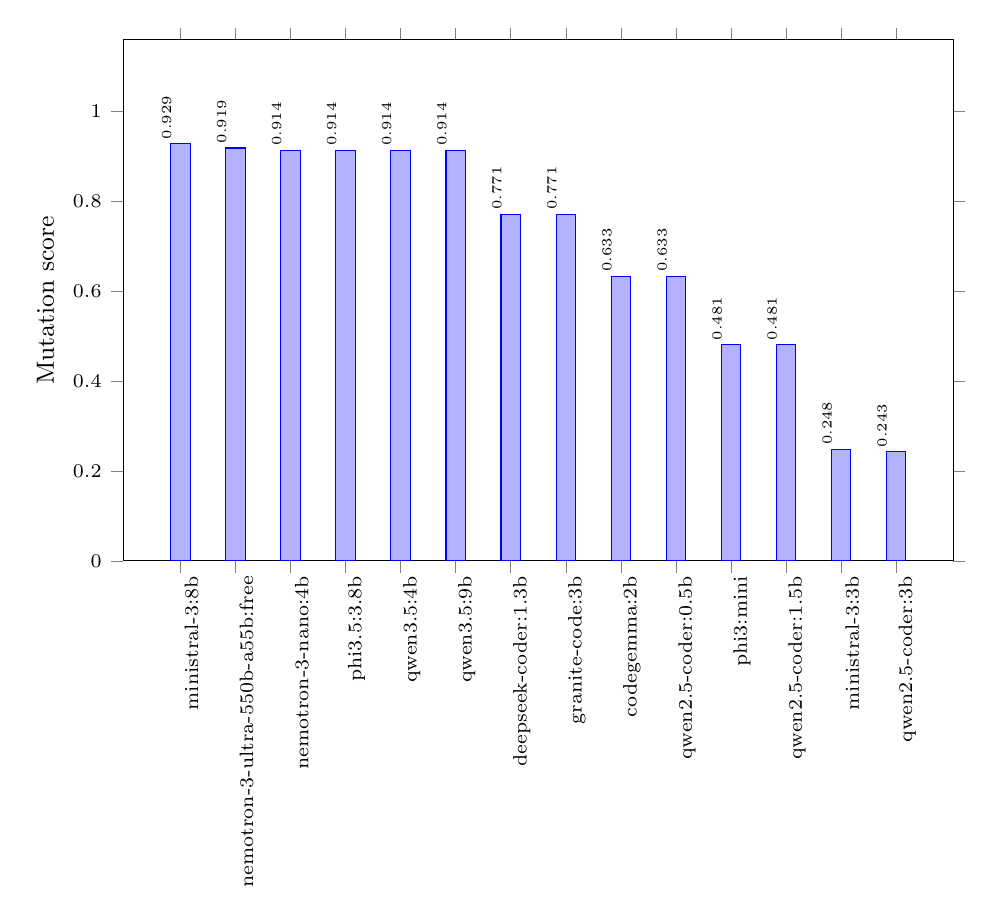
\begin{tikzpicture}
\begin{axis}[
  ybar,
  bar width=7pt,
  bar shift=0pt,
  width=\textwidth,
  height=8.2cm,
  ylabel={Mutation score},
  xtick={0,1,2,3,4,5,6,7,8,9,10,11,12,13},
  xticklabels={ministral-3:8b,nemotron-3-ultra-550b-a55b:free,nemotron-3-nano:4b,phi3.5:3.8b,qwen3.5:4b,qwen3.5:9b,deepseek-coder:1.3b,granite-code:3b,codegemma:2b,qwen2.5-coder:0.5b,phi3:mini,qwen2.5-coder:1.5b,ministral-3:3b,qwen2.5-coder:3b},
  x tick label style={rotate=90, anchor=east, font=\scriptsize, inner sep=1pt, yshift=-4pt},
  y tick label style={font=\scriptsize},
  label style={font=\small},
  ymin=0,
  ymax=1.160000,
  enlarge x limits=0.08,
  tick align=outside,
  clip=false,
]
\addplot+[bar shift=0pt] coordinates {(0,0.928571) (1,0.919048) (2,0.914286) (3,0.914286) (4,0.914286) (5,0.914286) (6,0.771429) (7,0.771429) (8,0.633333) (9,0.633333) (10,0.480952) (11,0.480952) (12,0.247619) (13,0.242857)};
\addplot[
  only marks,
  mark=none,
  bar shift=0pt,
  forget plot,
  nodes near coords,
  point meta=explicit symbolic,
  every node near coord/.append style={font=\tiny, rotate=90, anchor=west, inner sep=1.5pt, yshift=5pt, fill=white, fill opacity=0.9, text opacity=1},
] table[x=x,y=y,meta=label] {
x y label
0 0.928571 {0.929}
1 0.919048 {0.919}
2 0.914286 {0.914}
3 0.914286 {0.914}
4 0.914286 {0.914}
5 0.914286 {0.914}
6 0.771429 {0.771}
7 0.771429 {0.771}
8 0.633333 {0.633}
9 0.633333 {0.633}
10 0.480952 {0.481}
11 0.480952 {0.481}
12 0.247619 {0.248}
13 0.242857 {0.243}
};
\end{axis}
\end{tikzpicture}
